\documentclass[conference]{IEEEtran}
\IEEEoverridecommandlockouts
\usepackage{cite}
\usepackage{amsmath,amssymb,amsfonts}
\usepackage{algorithmic}
\usepackage{graphicx}
\usepackage{textcomp}
\usepackage{xcolor}
\usepackage{hyperref}
\usepackage{placeins}
\usepackage[spanish, mexico]{babel}
\def\BibTeX{{\rm B\kern-.05em{\sc i\kern-.025em b}\kern-.08em
    T\kern-.1667em\lower.7ex\hbox{E}\kern-.125emX}}
\usepackage[table,xcdraw]{xcolor}

\title{Análisis de Sentimiento con Reseñas de IMDB}

\author{\IEEEauthorblockN{
Dora Alicia Guevara Villalpando \\
Matrícula: 1551003}
\\
\IEEEauthorblockA{\textit{Universidad Autónoma de Nuevo León)} \\
\textit{Facultad de Ciencias Físico Matemáticas}\\
Maestría en Ciencia de Datos \\
Procesamiento y Clasificación de Datos\\\\
dora.guevaravll@uanl.edu.mx}
}

\date{\today}

\begin{document}

\maketitle


\begin{abstract}
Este documento presenta un análisis de sentimientos en reseñas de películas utilizando el modelo VADER. Se preprocesa el texto mediante limpieza, lematización y eliminación de stopwords. Se comparan las predicciones del modelo con etiquetas originales para evaluar su desempeño. Los resultados indican que VADER es eficiente en la clasificación de sentimientos, pero presenta limitaciones en textos con lenguaje figurado o sarcasmo.
\end{abstract}



\section{Introducción}

El análisis de sentimientos es una técnica clave en el procesamiento de lenguaje natural (NLP) que permite determinar la polaridad emocional de un texto, clasificándolo en positivo, negativo o neutro. Este tipo de análisis es ampliamente utilizado en la minería de opiniones para evaluar reseñas de productos, películas y servicios.

En este proyecto, se analiza un conjunto de datos de reseñas de películas de \textbf{IMDb} utilizando la herramienta VADER (Valence Aware Dictionary and sEntiment Reasoner), que se basa en un diccionario de palabras con asignación de polaridad para identificar la intensidad del sentimiento. El objetivo principal es comparar la precisión del análisis de sentimientos automático con las etiquetas de clasificación originales del conjunto de datos.

El informe presenta el procesamiento de los datos, la metodología utilizada, los resultados obtenidos y las conclusiones basadas en el rendimiento del modelo de análisis de sentimientos.




\section{Descripción del Conjunto de Datos}

El conjunto de datos utilizado en este estudio es el \textbf{Large Movie Review Dataset v1.0}, desarrollado por Andrew L. Maas et al. (2011) y publicado en la conferencia \textbf{ACL-HLT 2011}. Este dataset es ampliamente utilizado como referencia en tareas de clasificación de sentimientos y contiene reseñas de películas etiquetadas con polaridad positiva o negativa.

\subsubsection{Características del dataset}

\begin{itemize}

	\item Contiene 50,000 reseñas etiquetadas de manera balanceada en 25,000 positivas y 25,000 negativas. Se divide en:
		\begin{itemize}
		\item 25,000 reseñas de entrenamiento (12,500 positivas y 12,500 negativas).
		\item 25,000 reseñas de prueba (12,500 positivas y 12,500 negativas).
		\end{itemize}
	
	\item Cada reseña proviene de una película diferente para evitar sesgos de correlación.
	
	\item Solo se incluyen reseñas con calificaciones extremas:
		\begin{itemize}
		\item Positivas: Puntuaciones $ \geq 7 $ en IMDb.
		\item Negativas: Puntuaciones $ \leq 4 $ en IMDb.
		\item Las reseñas con calificaciones neutrales no están incluidas en los conjuntos de entrenamiento y prueba.
		\end{itemize}
	
	\item Se incluyen 50,000 reseñas sin etiquetas para estudios de aprendizaje no supervisado.
	
\end{itemize}

El dataset está estructurado en carpetas train/ y test/, con subdirectorios pos/ y neg/ que contienen los archivos de texto con las reseñas y sus respectivas etiquetas.


\section{Planteamiento del Problema}

El análisis de reseñas de películas proporciona información valiosa sobre la percepción del público y su experiencia con una producción cinematográfica. Sin embargo, el proceso manual de clasificación es costoso y subjetivo, lo que resalta la necesidad de utilizar modelos automáticos de análisis de sentimientos.

Este estudio busca responder la siguiente pregunta:

\textit{¿Qué tan precisa es la herramienta VADER en la clasificación de reseñas de películas en comparación con las etiquetas originales?}

Para responder estas preguntas, se implementa un pipeline de preprocesamiento de texto y se comparan los resultados del análisis de sentimientos automático con las etiquetas originales del dataset.



\section{Metodología}

\subsection{Carga del Conjunto de Datos}

Se descargó el dataset \textit{Large Movie Review Dataset v1.0} desde la fuente oficial y se almacenó en un DataFrame con dos columnas: \textbf{review} (texto) y \textbf{sentiment} (etiqueta original: 1 = positivo, 0 = negativo).


\subsection{Preprocesamiento del Texto}

Los pasos de limpieza incluyen:
\begin{enumerate}
    \item Eliminación de etiquetas HTML con \textit{BeautifulSoup}.
    \item Eliminación de caracteres no alfanuméricos.
    \item Tokenización y conversión a minúsculas.
    \item Lematización con WordNet.
    \item Eliminación de \textit{stopwords} en inglés.
\end{enumerate}


\subsection{Análisis de Frecuencia de Palabras}

Se realizó un análisis para obtener las palabras más frecuentes utilizadas en los reviews  después del preprocesamiento del texto.


\subsection{Análisis de Sentimientos}

Se utilizó el modelo VADER para clasificar cada reseña:
\begin{itemize}
    \item \textbf{Positivo}: $compound \geq 0$
    \item \textbf{Negativo}: $compound < 0$
\end{itemize}

Se almacenó el resultado en la columna \texttt{predicted\_sentiment}


\subsection{Evaluación del Modelo}

Para comparar las etiquetas originales con las predicciones del modelo, se usaron:
\begin{itemize}
    \item \textbf{Matriz de Confusión}: Muestra aciertos y errores de clasificación.
    \item \textbf{Precisión Global}: Porcentaje de predicciones correctas.
    \item \textbf{Reporte de Clasificación}: Análisis de precisión, recall y F1-score.
\end{itemize}



\section{Análisis de Resultados}

\subsection{Frecuencia de palabras}

Se obtuvo el top 20 de las palabras con mayor frecuencia entre todos los reviews. En este se observó que las palabras más usadas en los reviews son: \texttt{movie, film, one, like, time, good}, entre otras. 

En la  Figura~\ref{fig:frecuencia_palabras_top20} se observa el listado completo del top 20 de palabras más usadas,


\subsection{Precisión del Modelo}

\begin{itemize}
    \item \textbf{Precisión Global}: 66.96\% de aciertos.
    \item \textbf{Negativo}:
        \begin{itemize}
            \item Precisión: 79\%
            \item Recall: 46\%
        \end{itemize}
    \item \textbf{Positivo}:
        \begin{itemize}
            \item Precisión: 62\%
            \item Recall: 88\%
        \end{itemize}
\end{itemize}


\subsection{Matriz de Confusión}

Acorde a los resultados mostrados en la Figura~\ref{fig:matriz_confusion} podemos decir lo siguiente:

\begin{itemize}
	\item El modelo cometió más errores al clasificar reseñas negativas como positivas. 
	\item La ausencia de una categoría ''Neutro'' en el dataset original pudo afectar la precisión.
\end{itemize}



\subsection{Análisis de Discrepancias}

Se encontraron discrepancias en reseñas con:
\begin{itemize}
    \item \textbf{Sarcasmo}: ''I love wasting my time watching this.''
    \item \textbf{Doble sentido}: ''This movie was \textbf{too good} to be true.''
    \item \textbf{Expresiones ambiguas}: ''Not bad at all'' fue clasificado erróneamente como negativo.
\end{itemize}



\section{Conclusiones}

\begin{itemize}
    \item \textbf{VADER es eficiente en la clasificación de sentimientos}, pero presenta errores en textos con subjetividad o sarcasmo.
    \item \textbf{El modelo tiene un sesgo hacia lo positivo}, lo que genera falsos positivos en reseñas negativas.
    \item \textbf{El preprocesamiento es clave}, pero la eliminación de stopwords puede afectar frases con negaciones sutiles.
    \item \textbf{Se recomienda el uso de modelos más avanzados}, como BERT o transformers, para mejorar la precisión en textos con lenguaje complejo.
\end{itemize}




\begin{thebibliography}{9}
    \bibitem{maas2011learning} Maas, A. et al. (2011). \textit{Learning Word Vectors for Sentiment Analysis}. ACL-HLT 2011. URL: \url{http://www.aclweb.org/anthology/P11-1015}.
    \bibitem{potts2011negativity} Potts, C. (2011). \textit{On the negativity of negation}. Semantics and Linguistic Theory 20, 636-659.
    \bibitem{imdbdataset} IMDB Movie Reviews Dataset. URL: \url{https://ai.stanford.edu/~amaas/data/sentiment/}.
    \bibitem{scikit-learn} Scikit-learn Library (TF-IDF, Logistic Regression, SVM, Random Forest). URL: \url{https://scikit-learn.org/}.
    \bibitem{textmining} Análisis de texto (text mining) con Python. URL: \url{https://cienciadedatos.net/documentos/py25-text-mining-python}.
\end{thebibliography}

\newpage 
\onecolumn

\section{Anexo: Gráficos.}


\begin{figure}[h]
    \centering
    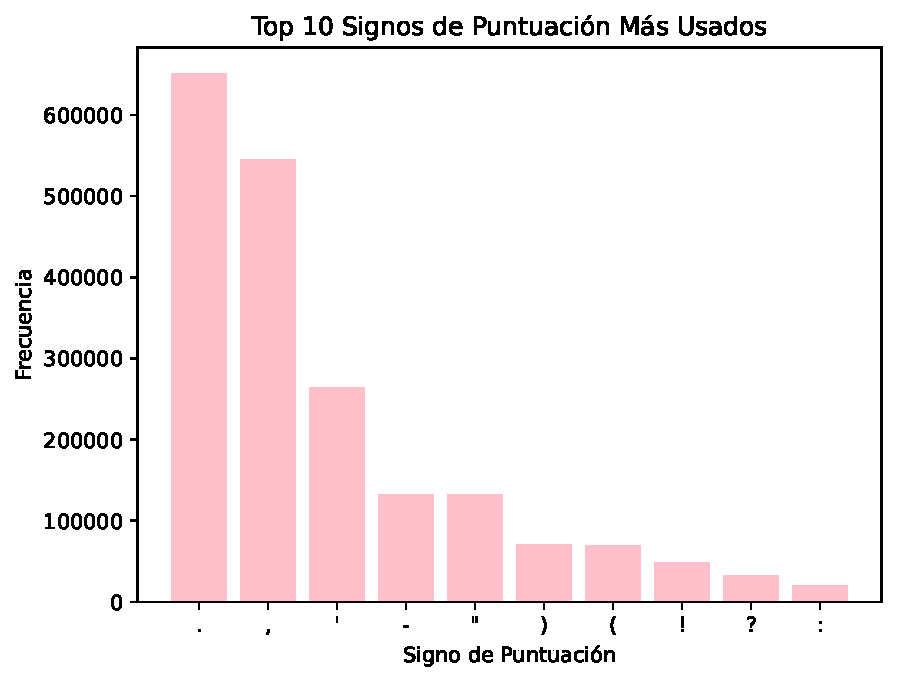
\includegraphics[width=.8\textwidth]{imagenes/signos_puntuacion.pdf}
    \caption{Gráfico del top 10 de los signos de puntuación mas usados.}
    \label{fig:signos_puntuacion}
\end{figure}

\FloatBarrier

\begin{figure}[h]
    \centering
    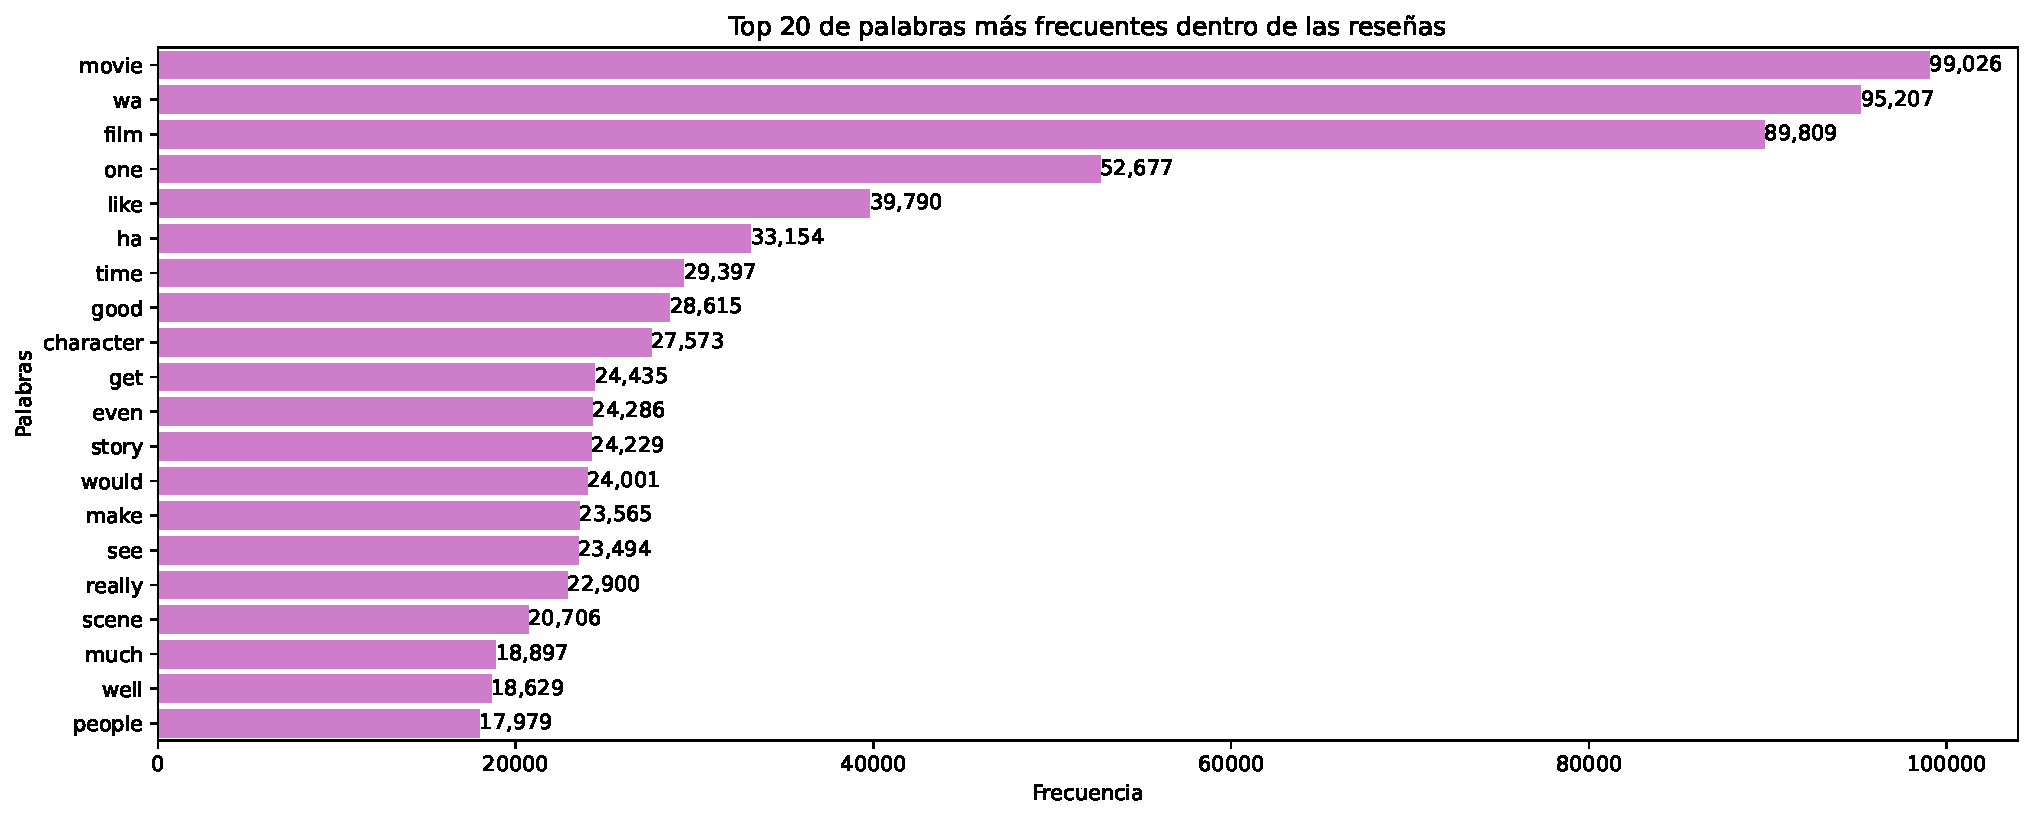
\includegraphics[width=1\textwidth]{imagenes/frecuencia_palabras_top20.pdf}
    \caption{Gráfico del top 20 palabras mas frecuentes.}
    \label{fig:frecuencia_palabras_top20}
\end{figure}


\begin{figure}[h]
    \centering
    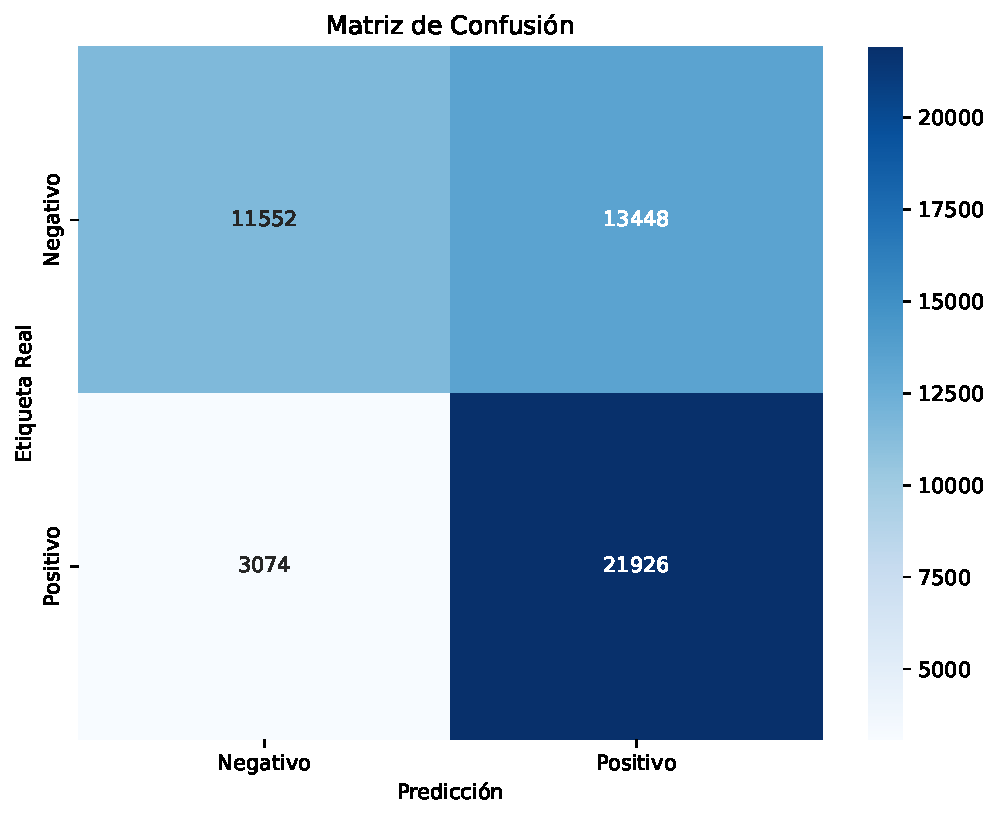
\includegraphics[width=.8\textwidth]{imagenes/matriz_confusion.pdf}
    \caption{Matriz de Confusión.}
    \label{fig:matriz_confusion}
\end{figure}




\end{document}